% !TeX spellcheck = en_GB
% CNN explanation

\label{section:cnn}

	One of the most explored implementations is the one related to \acrfull{cnn}. This maintain the basic idea of receiving some inputs and apply a dot product operation to them before subject the data to a non-linear function but with the difference that input data are expected to be images \cite{Karpathy2016}. The architecture of a \acrlong{convnet} is based on the organization of the Visual Cortex in the human brain. This means that single neurons responds to some stimuli only in a certain region of the visual field, the Receptive Field. Then, a collection of these fields overlap with each other so as to cover the full visual space \cite{Saha2018}.
	
	About the input data, it is introduced as a matrix instead of as a row vector. Then, the architecture of the layers adapt to the fact that input data are images. They do not consist of a single row of neurons, but they have a shape constituted by three dimensions: heigh, width and depth \cite{Karpathy2016} \todo{include image?}. In this way, the net can capture the spatial and temporal relations present in an image by applying some filter functions. With this construction, the model can be trained with a smaller number of parameters and also reuse the weights.
	
	A \acrlong{convnet} can be described as a sequence of layers in which every layer converts a volume of activation results from the previous layer to another by computing a differentiable function. The architecture of a \acrshort{cnn} is always composed by three type of distinguishable layers which are \textit{Convolutional}, \textit{Pooling} and \textit{\acrlong{fc}}. A normal architecture will follow the next succession of layers \cite{Karpathy2016}:
	
	\begin{itemize}
		\item INPUT: this represents the image at the entrance of the whole model. It commonly is a 3\acrshort{d} matrix , one dimension per channel of colour, and contains the values of the original pixels.
		\item CONVOLUTIONAL: considering the neurons that are connected to a region of the input image, this layer computes their output by performing a dot product between the weights and the value of the pixels. The depth of the resulting data will coincide with the number of filters used.
		\item POOL: this performs a fixed operation that consists of a downsampling of the spatial dimension. It typically reduces by half the height and the width of the input image.
		\item \acrshort{fc}: this is the final layer which gives the output of the whole net. It is a vector-shape layer and is completely connected to the previous layer. In a classification task the number of neurons matches the amount of classes of the problem.
	\end{itemize}
	
	Note that this list represents the order of the layers in the architecture, however, the number of layers of each type vary depending on how the model is designed and how deep it is desired to be. For example, some examples of deep architectures can be found later in section \ref{subsection:vgg}, in table \ref{table:3}.
	
	With this building, a \acrlong{convnet} passes the information of the pixels layer by layer while reducing the input images in a way that is much easier to process. This is performed without missing any feature since all of them are essential to compute a good prediction outcome.
	
	In the convolutional layer, a convolution operation is performed for each small region of the input image. The element that carries out this operation is called \textit{kernel} or \textit{filter}. This partial region that the kernel covers in the input data is set by deciding the height and the width as a designing parameter. About the depth, it must match the depth of the input data so the filter can slide trough the image along its 2\acrshort{d} and obtaining the results of the convolution operation by computing between the pixels inside the region and the values of the filter. An example can be observed in figure \ref{fig:mesh11}. For each filter, a 2\acrshort{d} activation map is obtained after subjected the result of the convolution to a non-linear operation as the \acrfull{relu} function. Finally, we will pack all these in a unique volume that will consists in the output of the convolutional layer \cite{Karpathy2016}. For example, if we have a number of 64 filters, we will get then a group of 64 2\acrshort{d} activation maps that will be the input of the next layer. Traditionally, it was the first convolutional layer the one that was responsible of capturing low-level features related to edges or colours in the image. The upper layers were the ones in charge of extracting high-level features so the network was able to understand the image similar to how the humans do \cite{Saha2018}.
	
	\begin{figure}[ht]
		\centering
		\captionsetup{justification=centering}
		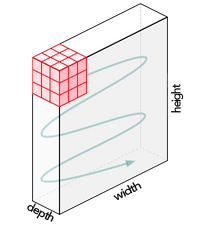
\includegraphics[scale=0.6]{movement-of-kernel}
		\caption{Movement of the kernel represented as a red block along the width and the height of the original input image. It is clear that it occupies the whole depth of the input image. The arrow indicates an approximation of the movement that the filter follows \cite{Saha2018}.}
		\label{fig:mesh11}
	\end{figure}

	We have included how the input interacts with the convolutional layer and also introduced the concept of depth of the resulting volume. However, it is needed to explain the how the total size of this output is computed and what it depends on. There are three main parameters that play a role in this decision: \textit{depth}, \textit{stride} and the \textit{zero-padding} \cite{Karpathy2016}.
	
	\begin{itemize}
		\item DEPTH: it is a hyperparameter that corresponds to the amount of kernels used in the convolutional layer when learning from the input.  The set of neurons that extent through the depth dimension operating in the same region is called depth column. This is the previous mentioned red block shown in figure \ref{fig:mesh11}.
		\item STRIDE: this indicates the displacement of the sliding filter along the image. If it has a value of 1 (non-strided), this means that the kernel will shift a position of one pixel along the width. When it is set to 2, then it moves two pixels. It rarely has values greater than 2. The moving process consists on the filter going from right to left with a hop determined by the stride value. When the right margin is reached, then it jumps to the beginning of the next row from the left margin and repeats the process in the same way until the image is completed \cite{Saha2018}. The bigger the stride, the smaller the size of the output volume.
		\item ZERO-PADDING: this is also called just \textit{padding}. It consists on adding zeros to the borders of the image. What is a hyperparameter in design is the size of this padding. This allows to control the width and height of the output volume so we can keep it the same through the different layers. When it is indicate a "valid padding", it means that no padding is added and the output size will be reduced. If we indicate "same padding", then it has a value of 1 and means that the resulting volume will have the size of the input \cite{Keras}.
	\end{itemize}

	As shown below, the total size of the obtained volume, $D$, can be computed as function of the input size, $W$, the spatial 2\acrshort{d} dimensions of the convolutional filter, $F$, the stride of the filters shifting, $S$,  and the amount of padding in the zero-padding, $P$ \cite{Karpathy2016}. 
	
	\[ D = \frac{W - F + 2P}{S} + 1 \]
	
	The convolutional layers can be grouped all together, one after another, but they are usually interpolated by what it has been previously defined as \textit{pooling} layer. This habit has the objective of reducing the the width and the height of the resulting volumes in a progressive manner in order to decrease the total number of training parameters and control the computational cost, and, therefore to avoid overfitting \cite{Karpathy2016} \todo{Include definition of overfitting or just cite it}. There can be performed two types of pooling operation: the max-pooling or the average-pooling. The former just returns the maximum value from the portion of the image where the filter is placed. The latter, computes the average of all the values in this portion \cite{Saha2018}. The pooling layer acts in an independent way on every input depth level. 
	
	Two hyperparameters are needed in order to configure the spatial portion in which the pooling is computed: the  filter size, related to length of height and width, and the stride. However, for this operation zero parameters are introduce since it consists on a fixed operation over the input data. In figure \ref{fig:mesh12}, it is shown how the max-pooling operation is performed \cite{Karpathy2016}. 
	
	\begin{figure}[ht]
		\centering
		\captionsetup{justification=centering}
		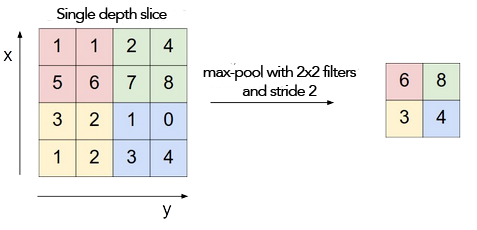
\includegraphics[scale=0.7]{max-pooling}
		\caption{Max-pooling operation with a filter size of 2 and a stride of 2 for a single depth filter. Each colour represents a the action portion for each operation \cite{Karpathy2016}}
		\label{fig:mesh12}
	\end{figure}
	
	Together a convolutional layer and a pooling layer constitute a complete layer structure typical in a \acrlong{convnet}. The number of these complete layers can vary depending on the design and the task needs. These represent the main core of the network before passing to the last layers and calculating the final output \cite{Saha2018}.
	
	For the final step, a common way of acting is to apply some non-linear activations in order to learn from the high-level features resulted from the output volume of the last convolutional layer. This takes place in the \acrlong{fc} layers ending the model. This part has the shape of a Fully-Connected layer, as the one described in the basic model of \acrshort{ann}. To make the weights from the convolutional layers available to feed this last part of the model, it is necessary to flatten the output volume and obtain a column vector. The learning process is possible due to a backpropagation operation performed in every epoch of training. As a total output, the values that represent the classification of the different samples into one or another category are obtained \cite{Saha2018}. A common classification technique is the one called \textit{Softmax}. This normalizes the result of the previous \acrshort{fc} layer into a vector whose values follow a distribution that total sum results in 1. This type of output is called \textit{soft predictions} and represent the probability for each sample of belonging to a category in the classification \cite{Mahmood2018}. However, there exists other activation functions that can compute the classification output in other ways. 
	
	In figure \ref{fig:mesh13} an scheme of a common \acrlong{cnn} is shown. This takes an input image, compute the features along three groups of convolutional layer plus max-pooling and, finally, includes three \acrlong{fc} layers, being the last one a softmax function layer with as many neurons as classes that gives the soft predictions for this image of belonging to each class.
	
	\begin{figure}[ht]
		\centering
		\captionsetup{justification=centering}
		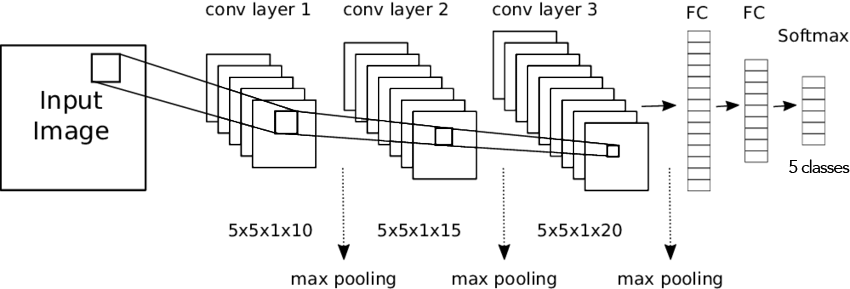
\includegraphics[scale=0.4]{cnn}
		\caption{Representation of a typical CNN model \cite{Hinz2016}}
		\label{fig:mesh13}
	\end{figure}

	\acrfull{cnn} were originally designed to work with images but they have been applied to other fields as audio. An image can be defined as a matrix of values, i.e. pixels, in two or three dimensions, so the only prerequisite to use a \acrshort{cnn} is to have the input data in this form. For audio researching, it has been commonly used the log-scaled mel spectrogram, that is a way of representing audio in a scale different than frequency that is more similar to humans perception. It has been used in plenty of works with \acrshort{cnn} and also combined with other techniques \cite{Salamon2017} \cite{Piczak2015} \cite{Kumar2017}.
	
	
	

	

	
	
	
	
	